% 1977 年安徽卷（理科）第 9 题（附加题）：矩形 ABCD 分割示意图，
% AD 边上 A1—A4 五等分（AA1=…=A4D=a），AB 边上 B1、B2 三等分（AB1=B1B2=B2B=√3a），
% 过 A1 作 AB 的平行线交 BC 于 G，E 在该线上 B1 的正上方（B1E⊥AB），
% 连线 A1B1、A1B2（按源卷第 4 页「安，加．」手绘图布局重绘）
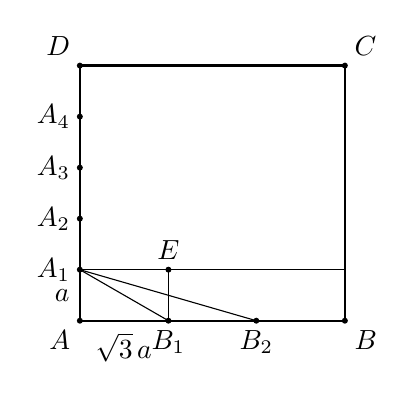
\begin{tikzpicture}[scale=0.9]
  \coordinate (A) at (0,0);
  \coordinate (B) at (3.74,0);
  \coordinate (C) at (3.74,3.6);
  \coordinate (D) at (0,3.6);
  \coordinate (A1) at (0,0.72);
  \coordinate (A2) at (0,1.44);
  \coordinate (A3) at (0,2.16);
  \coordinate (A4) at (0,2.88);
  \coordinate (B1) at (1.25,0);
  \coordinate (B2) at (2.49,0);
  \coordinate (E) at (1.25,0.72);
  \coordinate (G) at (3.74,0.72);
  \draw[thick] (A)--(B)--(C)--(D)--cycle;
  \draw[thin] (A1)--(G);
  \draw[thin] (A1)--(B1);
  \draw[thin] (A1)--(B2);
  \draw[thin] (B1)--(E);
  \fill (A) circle (1.2pt) node[below left] {$A$};
  \fill (B) circle (1.2pt) node[below right] {$B$};
  \fill (C) circle (1.2pt) node[above right] {$C$};
  \fill (D) circle (1.2pt) node[above left] {$D$};
  \fill (A1) circle (1.2pt) node[left] {$A_1$};
  \fill (A2) circle (1.2pt) node[left] {$A_2$};
  \fill (A3) circle (1.2pt) node[left] {$A_3$};
  \fill (A4) circle (1.2pt) node[left] {$A_4$};
  \fill (B1) circle (1.2pt) node[below] {$B_1$};
  \fill (B2) circle (1.2pt) node[below] {$B_2$};
  \fill (E) circle (1.2pt) node[above] {$E$};
  \node at (0.62,-0.38) {$\sqrt3\,a$};
  \node at (-0.25,0.36) {$a$};
\end{tikzpicture}
